\documentclass[12pt,a4paper]{article}
\usepackage{fullpage}
\usepackage[top=2cm, bottom=4.5cm, left=2.5cm, right=2.5cm]{geometry}
\usepackage{amsmath,amsthm,amsfonts,amssymb,amscd}
\usepackage{lastpage}
\usepackage{enumerate}
\usepackage{fancyhdr}
\usepackage{mathrsfs}
\usepackage{xcolor}
\usepackage{graphicx}
\usepackage{listings}
\usepackage{hyperref}
\usepackage{txfonts}
\usepackage{titlesec}
\usepackage{float}
\usepackage{esint}


\hypersetup{%
  colorlinks=true,
  linkcolor=blue,
  linkbordercolor={0 0 1}
}


\newcommand\course{8.03x - Vibrations and Waves}
\newcommand\hwnumber{1}               
\newcommand\MyName{Syed Suhaib Ahmad}
 
\renewcommand\lstlistingname{Algorithm}
\renewcommand\lstlistlistingname{Algorithms}
\def\lstlistingautorefname{Alg.}

\setlength{\parindent}{0.0in}
\setlength{\parskip}{0.05in}



\pagestyle{fancyplain}
\headheight 35pt
\lhead{\course}
\chead{\large\textbf{Problem Set 4}}
\rhead{\MyName{}}
\lfoot{}
\cfoot{\small\thepage}
\rfoot{}
\headsep 1.5em

\begin{document}

\subsubsection*{Problem 4.1 - Traveling pulse}
The figure shows a pulse on a string of length 100\,m with fixed ends. The pulse is traveling to the right without any change of shape, at a speed of 40\,m/sec.
\begin{figure}[h]
    \centering
    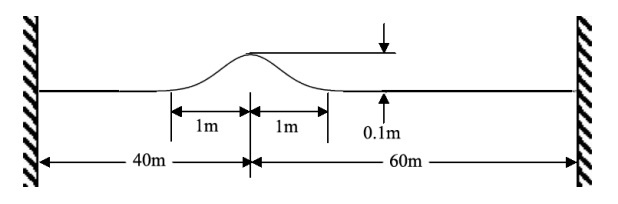
\includegraphics[width=0.6\linewidth]{figs/fig_prob_4.1.png}
    %\caption{Caption}
   % \label{fig:enter-label}
\end{figure}
\begin{enumerate}
    \item[(a)]Make a clear sketch showing how the transverse velocity of the string varies with distance along the string at the instant when the pulse is in the position shown.
    \item[(b)]What is the maximum transverse velocity of the string (approximately)?
    \item[(c)]If the total mass of the string is 2\,kg, what is the tension $T$ in it?
    \item[(d)]Write an equation for $y(x,t)$ that numerically describes sinusoidal waves of wavelength 5\,m and amplitude 0.2\,m traveling in the negative $x$ direction on a very long string made of the same material and under the same tension as above.
\end{enumerate}
\textbf{Solution(a)}
\begin{figure}[h!]
    \centering
    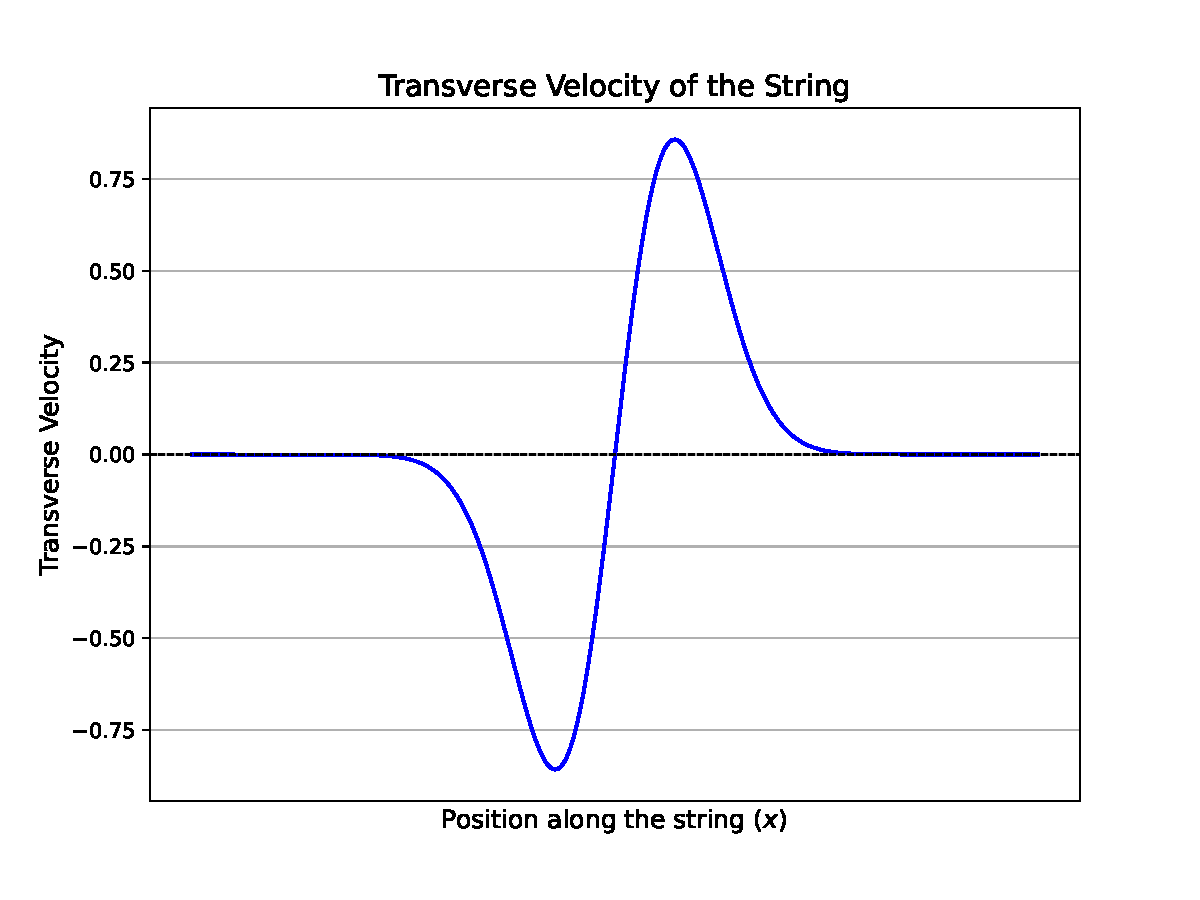
\includegraphics[width=0.879\linewidth]{figs/fig_sol_4.1a.pdf}
    %\caption{Caption}
    %\label{fig:enter-label}
\end{figure}
\newpage
\textbf{Solution(b)}
\\
\\The pulse resembles a bell curve, thus we can approximate it as a Gaussian function
\[y(\beta)=Ae^{-\alpha\beta^2},\]
where $\beta=x-vt$, $A=0.1\,$m and $\alpha=4\,\text{m}^{-2}$. The time derivative of $y(\beta)$ gives the transverse velocity.
\begin{equation}
    v_y=\frac{\partial y}{\partial t}=-2A\alpha\beta e^{-\alpha\beta^2}\frac{\partial\beta}{\partial t}=2Av\alpha\beta e^{-\alpha\beta^2}.
\end{equation}
Transverse velocity is maximum when
\[\frac{\partial^2y}{\partial t^2}=0\]
\[-2Av^2\alpha e^{-\alpha\beta^2}+4Av^2\alpha^2\beta^2e^{-\alpha\beta^2}=0\]
\[2Av^2\alpha e^{-\alpha\beta^2}\left(2\alpha\beta^2\right)=0.\]
At $t=0$, the above equation becomes
\[2Av^2\alpha e^{-\alpha x}\left(2\alpha x^2-1\right)=0\]
\[x=\sqrt{\frac{1}{2\alpha}}.\]
Upon substituting this value of $x$ and $t=0$ into Eq. (1), we get the maximum transverse velocity of the pulse at $t=0$.
\[v_{y\text{, max}}=2Av\sqrt{\frac{\alpha}{2}}e^{-1/2}\approx6.86\,\text{ms}^{-1}.\]
\textbf{Solution(c)}
\\
\\Velocity of the pulse is given by 
\[v^2=\frac{T}{\mu}\]
where $\mu$ is the mass density, which is $2/100=0.02\,\text{kgm}^{-1}$ for this rope. Thus, the tension is
\[T=\mu v^2=0.02\times40^2=32\,\text{N}.\]
\textbf{Solution(d)}
\\
\\Since the sinusoidal waves are traveling in the negative $x$ direction, the function describing them is of the form
\[y(x,t)=A\sin(kx+\omega t+\phi).\]
Same material and tension means its speed is same as the the speed of pulse, that is, $40\,$m/sec. Given that $k=2\pi/\lambda=2\pi/5\,\text{m}^{-1}$ and $\omega=kv=16\pi\,\text{s}^{-1}$. Amplitude $A$ of the waves is 2\,m. Thus the function defined above now becomes
\[y(x,t)=2\sin\left(\frac{2\pi}{5}x+16\pi t+\phi\right).\]
(Since no initial conditions are given, $\phi$ cannot be determined.)

\subsubsection*{Problem 4.2 - Traveling pulse}
A pulse traveling along a stretched string is described by the following equation:
\[y(x,t)=\frac{b^3}{b^2+(2x-ut)^2}\]
\begin{enumerate}
    \item[(a)]Sketch the graph of $y$ against $x$ for $t=0$.
    \item[(b)]What are the speed of the pulse and its direction of travel?
    \item[(c)]The transverse velocity of a given point of the string is defined by
    \[v_y=\frac{\partial y}{\partial t}\]
    Calculate $v_y$ as a function of $x$ for the instant $t=0$, and show by means of a sketch what this tells us about the motion of the pulse during a short time $\Delta t$.
\end{enumerate}
\textbf{Solution(a)}
\begin{figure}[h]
    \centering
    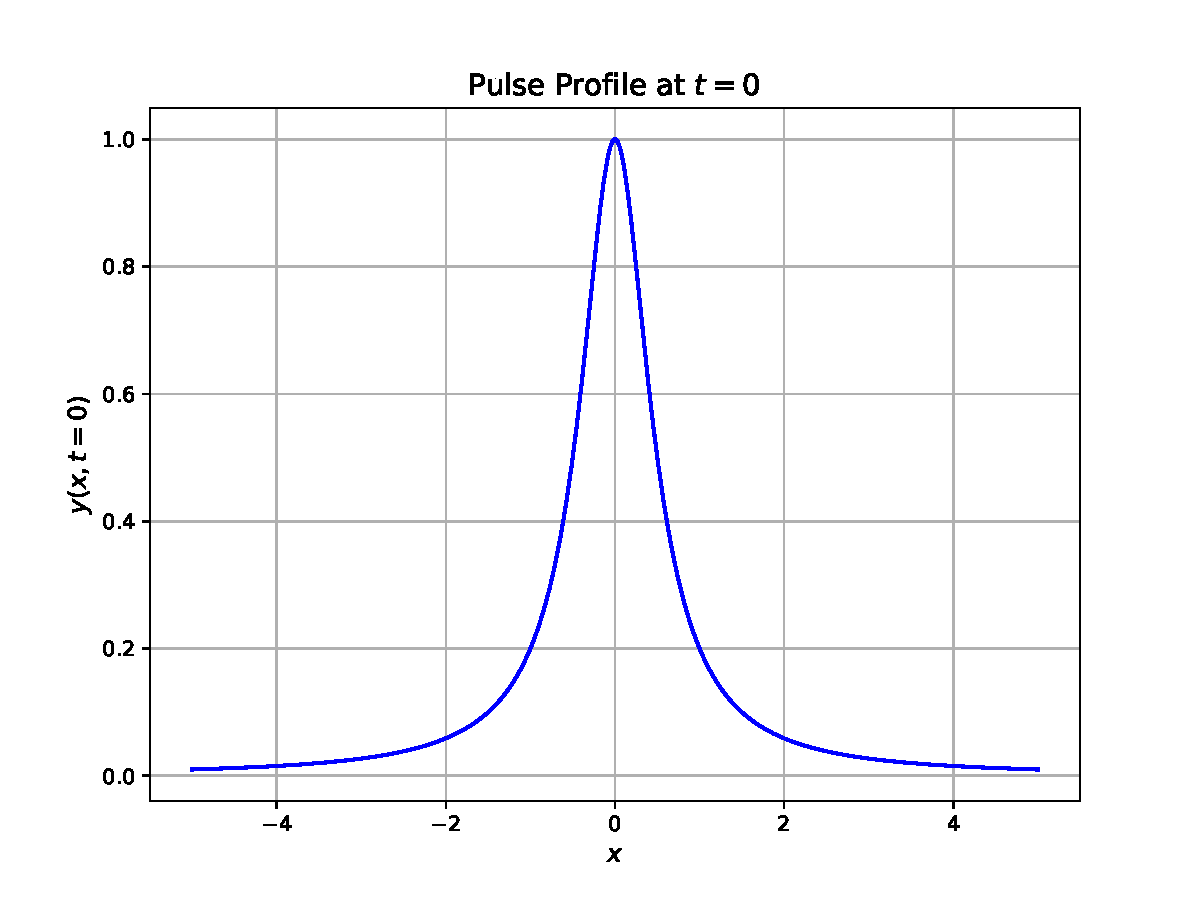
\includegraphics[width=0.879\linewidth]{figs/fig_sol_4.2a.pdf}
   % \caption{Caption}
  %  \label{fig:enter-label}
\end{figure}
\\\textbf{Solution(b)}
\\
\\Any traveling wave can be modeled by the function $f(\psi)$ where $\psi=kx\pm\omega t$. Thus, the given function is of the form
\[y(\psi)=\frac{b^3}{b^2+\psi^2}.\]
Since $\omega t$ is negative, the pulse is traveling in the negative $x$ direction. Speed of the pulse is given by the relation
\[v=\frac{\omega}{k}=\frac{u}{2}.\]
\textbf{Solution(c)}
\\
\begin{equation}
    v_y=\frac{\partial}{\partial t}\left(\frac{b^3}{b^2+(2x-ut)^2}\right)=\frac{2ub^3(2x-ut)}{\left(b^2+\left(2x-ut\right)^2\right)^2}.
\end{equation}
Equating Eq. (1) at $t=0$:
\[v_y=\frac{4xub^3}{\left(b^2+4x^2\right)^2}.\]
As the pulse is traveling in the positive $x$ direction, after a short time interval $\Delta t$, the pulse has shifted to right along the $x-$axis by a distance $(u/2)\Delta t$.
\begin{figure}[h]
    \centering
    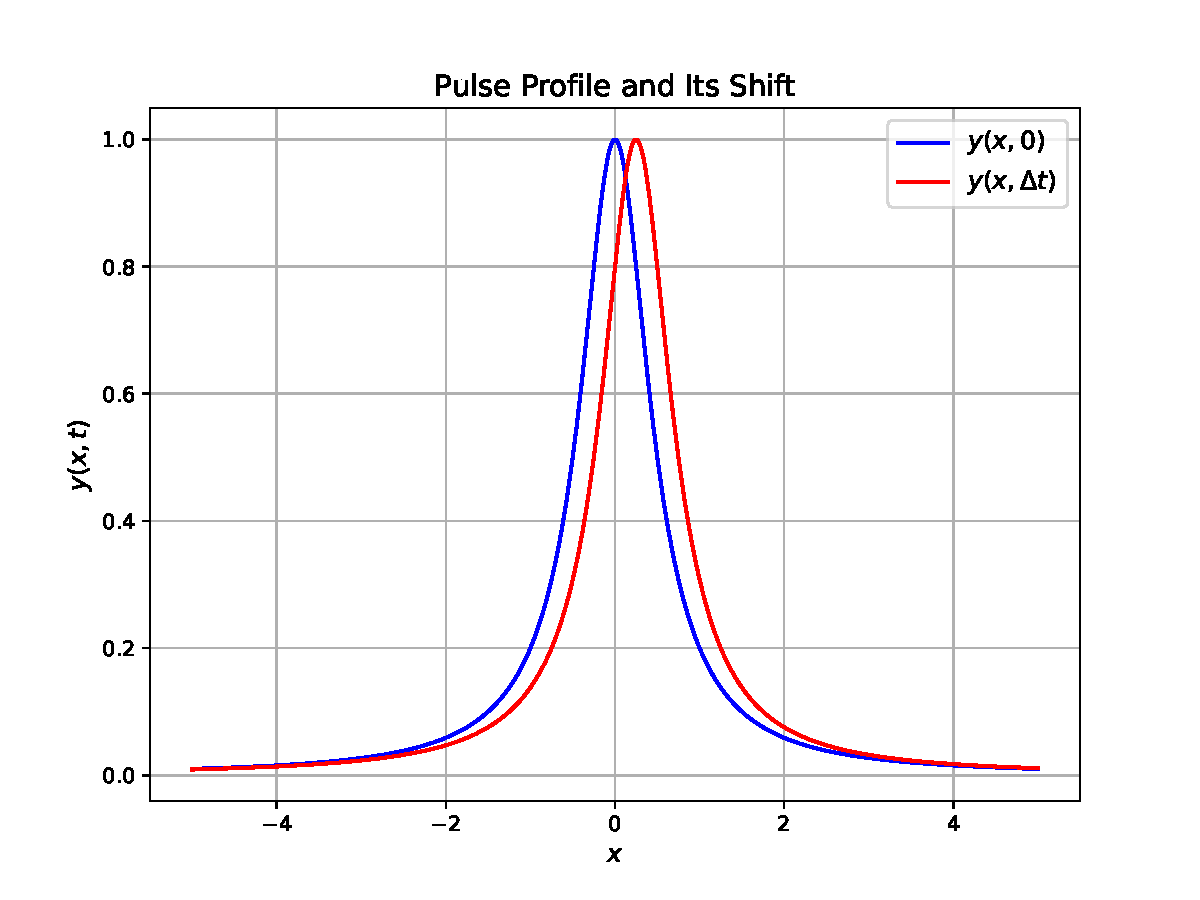
\includegraphics[width=0.879\linewidth]{figs/fig_sol_4.2c.pdf}
  %  \caption{Caption}
 %   \label{fig:enter-label}
\end{figure}
%\newpage
\subsubsection*{Problem 4.3 - Pulse reflection at a boundary }
Two strings with mass per unit length $\mu_1=0.1$\,kg/m and $\mu_2=0.3$\,kg/m, respectively, are jointed seamlessly. They are under tension $T=20$\,N. A traveling wave of a triangular shape shown in the figure is moving to the right along the lighter string. The tick marks set the scale of the pulse width.
\begin{figure}[h]
    \centering
    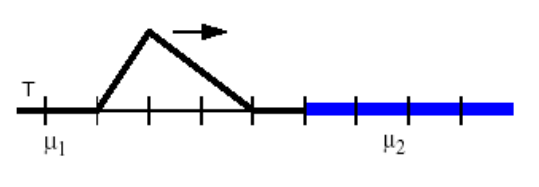
\includegraphics[width=0.6\linewidth]{figs/fig_prob_4.3.png}
    %\caption{Caption}
    %\label{fig:enter-label}
\end{figure}
\begin{enumerate}
    \item[(a)]Find the reflection and transmission coefficients at the interface (including the signs).
    \item[(b)]Make a careful sketch of the \textit{total} deformation of the string when the incident pulse has its peak exactly at the interface. Indicate how you arrived at your answer on your sketch.
    \item[(c)]Make a careful sketch of the \textit{total} deformation of the string when both the reflected and transmitted pulses have moved away from the interface.
    \item[(d)]What is unphysical about the shape of this pulse? (Be quantitative)
\end{enumerate}
\textbf{Solution(a)}
\\
\\Velocity of pulse in both media is given by $v_m=\sqrt{T/\mu_m}$. Thus the velocities ($\text{ms}^{-1}$) are
\[v_1=\sqrt{\frac{20}{0.1}}=10\sqrt{2}\,\,\,\,\,\text{and}\,\,\,\,\,v_2=\sqrt{\frac{20}{0.3}}=\frac{10\sqrt{6}}{3}.\]
The reflection and transmission coefficients can be determined using the following relationships
\begin{equation}
    R=\frac{v_2-v_1}{v_2+v_1}\,\,\,\,\,\text{and}\,\,\,\,\,T=\frac{2v_2}{v_1+v_2}.
\end{equation}
Substituting the values of $v_1$ and $v_2$ into the formulae given by Eq. (3) gives.
\[R=2-\sqrt{3}\approx0.25\,\,\,\,\,\text{and}\,\,\,\,\, T=-1+\sqrt{3}\approx0.75.\]
%\newpage
\textbf{Solution(b)}
\\
\\When the incident pulse reaches the interface, a reflected pulse (25\% of the incident pulse amplitude, with a sign inversion) is generated, and a transmitted pulse is created on the denser string. The transmitted pulse is narrower due to the reduced wave speed in the second medium. The total deformation at the boundary satisfies the displacement continuity condition:
\[y_\text{ref}+y_{\text{inc}}=y_{\text{trans}}.\]
The pulse shapes and their amplitudes obey the reflection and transmission coefficients determined by the wave impedance mismatch. While the displacement condition is satisfied exactly, the sharp corners of the triangular pulse may lead to an imperfect physical model, further discussed in part d.
\begin{figure}[H]
    \centering
    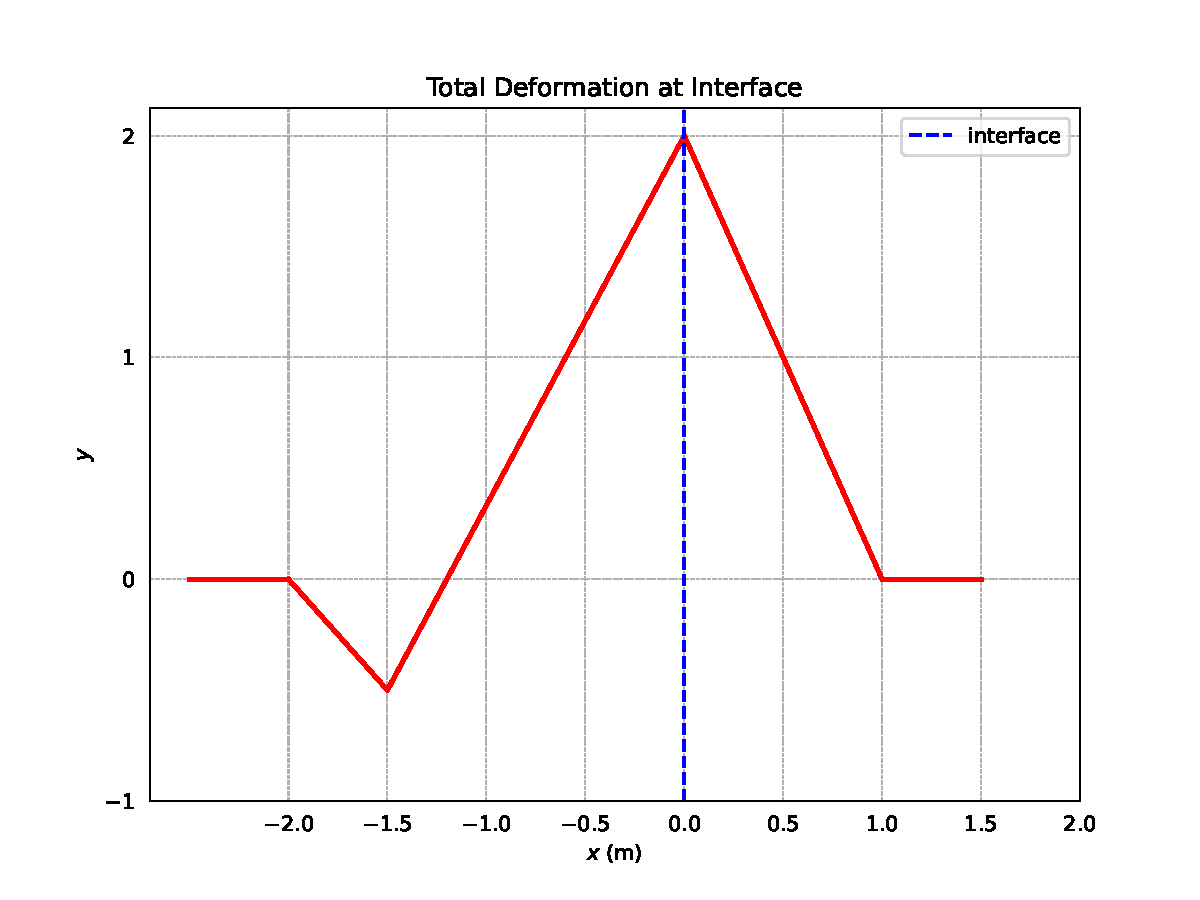
\includegraphics[width=0.9\linewidth]{figs/fig_sol_4.3b.pdf}
    \end{figure}
\textbf{Solution(c)}
\begin{figure}[H]
    \centering
    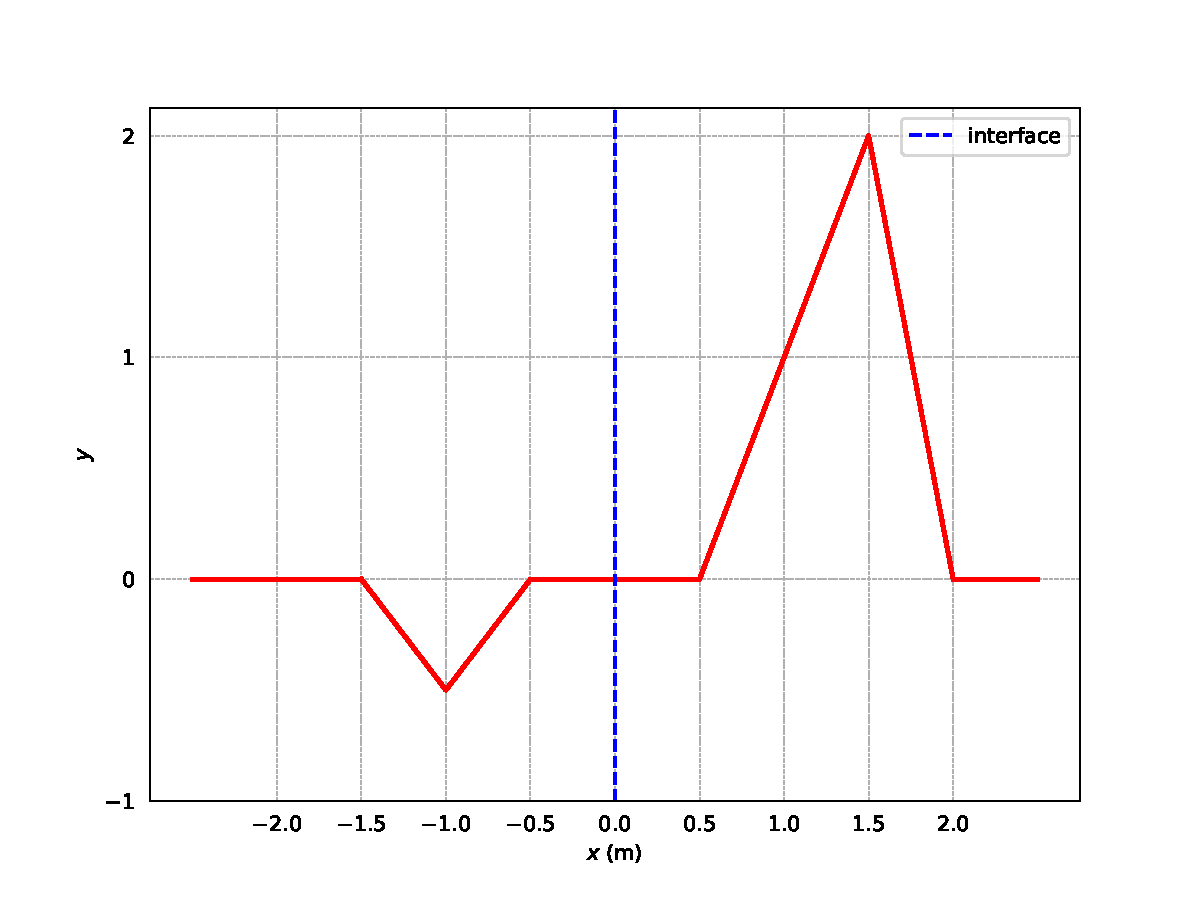
\includegraphics[width=0.9\linewidth]{figs/fig_sol_4.3c.pdf}
  %  \caption{Graphs for 4(b) and 4(c)}
\end{figure}

\textbf{Solution(d)}
\\
\\The discontinuity in the pulse due to this abrupt kink leads to infinite potential energy of the string. Potential energy of a string is given by the expression
\begin{equation}
    U=\int\frac{1}{2}T\left(\frac{\partial y}{\partial x}\right)^2\,dx,
\end{equation}
and since the slope is infinite at the point of discontinuity, the integral diverges to infinity. Furthermore, at any point in the string, the resultant force must be zero as each point has an infinitesimally small mass. Due to a sharp cusp in the string, there is always a component of tension acting at that point resulting in an infinite acceleration, which is not allowed in the model.

\subsubsection*{Problem 4.4 - Boundary conditions on a string}
A very long string of mass density $\mu$ and tension $T$ is attached to a small hoop with negligible mass. The hoop slides on a greased vertical rod and experiences a vertical force $F_y=-b\frac{\partial y}{\partial t}$ when it moves.
\begin{figure}[h]
    \centering
    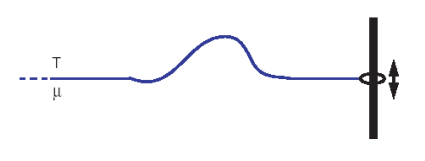
\includegraphics[width=0.6\linewidth]{figs/fig_prob_4.4.png}
    %\caption{Caption}
   % \label{fig:enter-label}
\end{figure}
\begin{enumerate}
    \item[(a)]Apply Newton’s law to the hoop to find the boundary condition at the end of the string. Express your result in terms of the partial derivatives of $y(x,t)$ at the location of the rod.
    \item[(b)]Show that the boundary condition is satisfied by an incident pulse $f(x-vt)$ and a reflected pulse $g(x+vt)$. Find $g$ in terms of $f$.
    \item[(c)]Show that your result has the correct behavior in the limits $b\rightarrow0$ (the string is free to slip) and $b\rightarrow\infty$ (the string is firmly clamped).
\end{enumerate}
\textbf{Solution(a)}
\\
\\By applying Newton's second law, we obtain
\begin{equation}
    \Delta m\frac{\partial^2x}{\partial t^2}=-T\sin\theta-b\frac{\partial y}{\partial t}.
\end{equation}
The small angle approximation can be used ($\sin\theta\approx\tan\theta\approx\frac{\partial y}{\partial x}$) assuming that the oscillations are small. Moreover, since the mass of hoop is negligible, $\Delta m\approx0$. Now, Eq. (5) can be rewritten as
\begin{equation}
    -T\frac{\partial y}{\partial x}-b\frac{\partial y}{\partial t}=0\Rightarrow\frac{\partial y}{\partial x}=-\frac{b}{T}\frac{\partial y}{\partial t}.
\end{equation}
Eq. (6) holds at the hoop for each and every value of $t$.
\\
\\\textbf{Solution(b)}
\\
\\Displacement continuity condition can be applied to the superposition of these two pulses.
\[y(x,t)=f(x-vt)+g(x+vt).\]
The spatial and time derivatives of the function $y(x,t)$ are
\[\frac{\partial y}{\partial x}=f'(x-vt)+g'(x+vt)\,\,\,\,\,\text{and}\,\,\,\,\,\frac{\partial y}{\partial t}=v\left(g'(x+vt)-f'(x-vt)\right).\]
Substituting the above results into Eq. (6) gives
\[f'(x-vt)+g'(x+vt)=-\frac{bv}{T}\left(g'(x+vt)-f'(x-vt)\right)\]
\[\frac{bv}{T}g'(x+vt)+g'(x+vt)=-f'(x-vt)+\frac{bv}{T}f'(x-vt)\]
\begin{equation}
    g'(x+vt)=\frac{bv/T-1}{bv/T+1x}f'(x-vt).
\end{equation}
Let the hoop is located at $x=0$. In this case, Eq. (7) simplifies to
\begin{equation}
    g'(vt)=\frac{bv/T-1}{bv/T+1}f'(-vt).
\end{equation}
For a subtle calculation, $vt$ can be substituted with a more general function $\Lambda$. Integrating Eq. (8) with respect to $\Lambda$ results in
\[g(\Lambda)=\frac{bv/T-1}{bv/T+1}\int f'(-\Lambda)\,d\Lambda=\frac{1-bv/T}{1+bv/T}f(-\Lambda).\]
It is important to note that the constant of integration must be zero otherwise the extreme cases discussed in next part will not hold.
\\
\\\textbf{Solution(c)}
\\
\\As $b\rightarrow0$, $g(\Lambda)=f(-\Lambda)$, which means that the pulse is reflected without flipping. This result very much intuitive as $b=0$ suggests that the hoop acts as a free end. Similarly, as $b\rightarrow\infty$, $g(\Lambda)=-f(-\Lambda)$. This suggests that the wave is reflected with a flip as $b=\infty$ means that the hoop acts as a clipped end. There is also a special case where $b=T/v$ and $g(\Lambda)=0$. This result is known as matched load whereby the incident pulse is terminated and the entirety of its energy is absorbed.

\subsubsection*{Problem 4.5 - Boundary conditions in a pipe}
Pressure oscillations in a hollow pipe of length $L$ are described by the wave equation
\[\frac{\partial^2p}{\partial z^2}=\frac{\rho_0}{\kappa}\frac{\partial^2p}{\partial t^2}\]
where $p$ is the over-pressure (over and above the one atmosphere ambient pressure), $\rho_0$ is the density of the gas in the pipe, $\kappa$ is the bulk modulus, and $z$ is the longitudinal direction along the pipe. Assuming a solution of the form
\[p(z,t)=[A\cos kz + B\sin kz]\cos\omega t\]
find all the unknowns ($A$, $B$, $k$ and $\omega$) for the case where the pipe is open at both ends and $p(z=L/2,t=0)=p_0$.
\\
\\\textbf{Solution}
\\
\\Firstly, we need to calculate the second spatial and time derivatives for the given solution.
\[\frac{\partial^2 p}{\partial z^2}=\left(-Ak^2\cos kz-Bk^2\sin kz\right)\cos\omega t\,\,\,\,\,\text{and}\,\,\,\,\,\frac{\partial^2 p}{\partial t^2}=-\omega^2\cos\omega t\left(A\cos kz + B\sin kz\right).\]

Now, we substitute these results into the wave equation.
\[\left(-Ak^2\cos kz-Bk^2\sin kz\right)\cos\omega t=-\frac{\rho_0}{\kappa}\omega^2\cos\omega t\left(A\cos kz + B\sin kz\right)\]
\[-Ak^2\cos kx\cos\omega t-Bk^2\sin kz\cos\omega t=-\frac{A\rho_0\omega^2}{\kappa}\cos kz\cos\omega t-\frac{B\rho_0\omega^2}{\kappa}\sin kz\cos\omega t\]
By comparing the coefficients, we obtain $k^2=\frac{\rho_0\omega^2}{\kappa}$.
\\
\\Given that the boundary conditions are $p(0,t)=0$ and $p(L,t)=0$.
\[p(0,t)=[A\cos0+B\sin0]\cos\omega t\Rightarrow A\cos\omega t=0.\]
The above calculation implies that $A=0$ since $p(0,t)$ should be zero for all values of $t$.
\\
\\$p(L,t)=0$ gives the following result:
\[\sin kL=0\Rightarrow k_n=\frac{n\pi}{L}\,\,\,\text{for}\,\,\,n=1,2,3...\]
This value of $k$ can be substituted into the expression derived earlier to obtain $\omega$.
\[\omega=\sqrt{\frac{\kappa k^2}{\rho_0}}\Rightarrow\omega_n=\frac{n\pi}{L}\sqrt{\frac{\kappa}{\rho_0}}.\]
Through the initial condition $p(z=L/2,t=0)=\rho_0$, we can determine $B$.
\[B\sin\left(\frac{n\pi}{2}\right)=\rho_0\Rightarrow B=\pm\rho_0\,\,\,\text{for}\,\,\,n=1,3,5...\]
Finally, $n$ must be an odd integer otherwise $p(z,t)$ would always be zero for even value of $n$, which is a trivial solution. Thus, the condition for $k$ should be modified. \[k_n=\frac{n\pi}{L}\,\,\,\text{for}\,\,\,n=1,3,5...\]

\subsubsection*{Problem 4.6 - Normal modes of discrete vs. continuous systems}
Referring to the diagram below, you are given a uniform string of length $L$ and total mass $M$ that is stretched to a tension $T$. You are also given a set of 5 beads, each of mass $M/5$, spaced at equal intervals on a massless string with tension $T$ and total length $L$.
\begin{figure}[h]
    \centering
    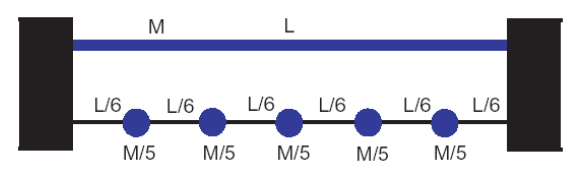
\includegraphics[width=0.6\linewidth]{figs/fig_prob_4.6.png}
   % \caption{Caption}
    %\label{fig:enter-label}
\end{figure}
\begin{enumerate}
    \item[(a)]Use boundary conditions to derive a general expression for the frequencies of the normal modes of oscillation of the string. Give the frequencies in terms of $n$, $T$, $L$ and $M$.
    \item[(b)]Write down the frequencies of the five lowest normal modes of transverses oscillation of the string.
    \item[(c)]Compare the numerical values of these normal mode frequencies with the normal mode frequencies of five beads on the massless string.
    \\\textit{Hint: You do not have to solve the frequencies of the beads. You may use French, eqns. 5-25 and 5-26.}
    \item[(d)]Sketch the five lowest normal modes you found for the massive string. Sketch also the five normal modes of the massless-string-with-five-beads.
    \item[(e)]In a sentence or two, discuss the differences, if any, in the normal modes of the two systems considered here.
\end{enumerate}
\textbf{Solution(a)}
\\
\\The most general solution for a standing wave is
\[y(x,t)=A\sin kx\cos\omega t.\]
The boundary conditions dictate that $y(0,t)$ and $y(L,t)$ are always zero. This leads to the result
\[A\sin kL=0\Rightarrow k=\frac{n\pi}{L}.\]
Therefore, the nth normal mode solution of the string is
\[y_n(x,t)=A_n\sin\left(\frac{n\pi}{L}x\right)\cos(\omega_nt).\]
Since the fundamental frequency $\omega_1=vk_1=v\pi/L$ (where $v=\sqrt{T/\mu}$ and $\mu=M/L$), the nth normal mode frequency is
\[\omega_n=n\omega_1=\frac{n\pi v}{L}=n\pi\sqrt{\frac{T}{ML}}.\]
General solution for nth mode can now be written as
\begin{equation}
    y_n=A_n\sin\left(\frac{n\pi}{L}x\right)\cos\left(n\pi \sqrt{\frac{T}{ML}}\,t\right)
\end{equation}
where the constant $A_n$ can be determined using the initial conditions.
\\
\\\textbf{Solution(b)}
\\
\\The frequency for the nth mode is given by
\[f_n=\frac{\omega_n}{2\pi}=\frac{n}{2}\sqrt{\frac{T}{ML}}.\]
It can be easily seen that each of the five lowest normal mode frequencies is an integer multiple of the fundamental frequency $f_0$.
\[f_1=\frac{1}{2}\sqrt{\frac{T}{ML}}=f_0,\,\,\,\,\,f_2=\sqrt{\frac{T}{ML}}=2f_0,\,\,\,\,\,f_3=\frac{3}{2}\sqrt{\frac{T}{ML}}=3f_0,\]
\[f_4=2\sqrt{\frac{T}{ML}}=4f_0,\,\,\,\,\,\text{and}\,\,\,\,\,f_5=\frac{5}{2}\sqrt{\frac{T}{ML}}=5f_0.\]
\textbf{Solution(c)}
\\
\\Frequency of each of the beads is given by \textit{French} Eq. (5-25).
\begin{equation}
    \omega_n=2\omega_0\sin\left(\frac{n\pi}{2(N+1)}\right)\Rightarrow f_n=\frac{\omega_0}{\pi}\sin\left(\frac{n\pi}{2(N+1)}\right).
\end{equation}
The fundamental for the beads is $\omega_0=\sqrt{\frac{T}{M/5\times L/6}}=\sqrt{120}f_0.$
\[f_1=\frac{\sqrt{120}f_0}{\pi}\sin\left(\frac{\pi}{12}\right)\approx0.9f_0,\,\,\,\,f_2=\frac{\sqrt{120}f_0}{\pi}\sin\left(\frac{\pi}{6}\right)\approx1.7f_0,\,\,\,\,\,f_3=\frac{\sqrt{120}f_0}{\pi}\sin\left(\frac{\pi}{4}\right)\approx2.5f_0,\]
\[f_4=\frac{\sqrt{120}f_0}{\pi}\sin\left(\frac{\pi}{3}\right)\approx3f_0,\,\,\,\,\,\text{and}\,\,\,\,\,f_5=\frac{\sqrt{120}f_0}{\pi}\sin\left(\frac{5\pi}{12}\right)\approx3.4f_0.\]
\newpage
\textbf{Solution(d)}
\\
\begin{figure}[h]
    \centering
    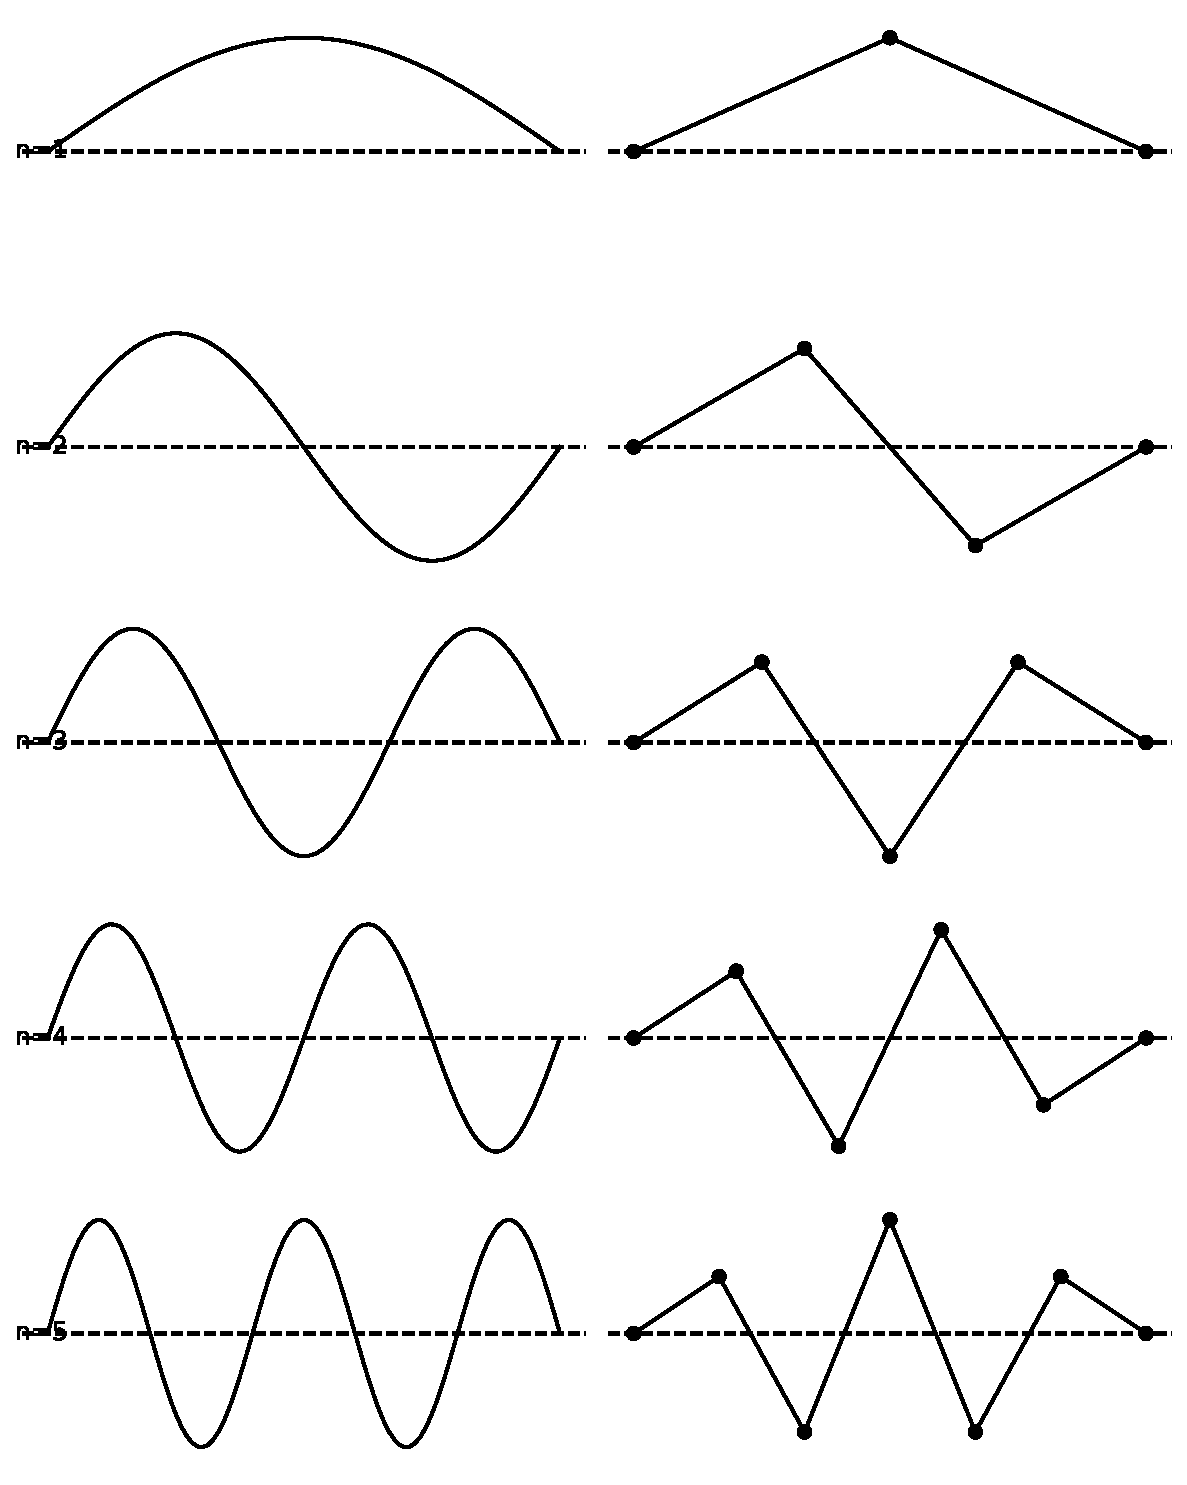
\includegraphics[width=0.9\linewidth]{figs/fig_sol_4.6d.pdf}
   % \caption{Enter Caption}
  %  \label{fig:enter-label}
\end{figure}
\\
\textbf{Solution(e)}
\\
\\The normal modes of the string system are continuous while the beads represent a discrete system. The nodes in the case of string occur at discrete points, with the displacement between the nodes following a sinusoidal fashion whereas in the case of beads, each bead oscillates with its own natural frequency.
\end{document}